\documentclass[final]{beamer}
\usepackage{amsmath,amssymb,amsthm,amsfonts,graphicx}
\usepackage{eulervm,verbatim}          
\usepackage[scaled]{helvet}
\usepackage[most]{tcolorbox}
\setbeamercolor{frametitle}{fg=black,bg=white} % Colors of the block titles
\setbeamertemplate{caption}{\raggedright\insertcaption\par}
\setbeamertemplate{caption}{\raggedright\insertcaption\par}
\definecolor{darkcerulean}{rgb}{0.03, 0.27, 0.49}
\newcommand{\citesmall}[1]{[{\color{darkcerulean}\begin{small} \textbf{#1} \end{small}}]}
\setbeamertemplate{footline}[frame number]
\DeclareMathOperator*{\argmin}{arg\,min}
\usepackage{graphicx}  % Required for including images
\usepackage{bbm}
\usepackage{booktabs} % Top and bottom rules for tables
\definecolor{burgundy}{rgb}{0.5, 0.0, 0.13}
\newcommand{\highlight}[1]{{\color{burgundy} \textbf{#1}}}
\usepackage{hyperref}
\hypersetup{
    colorlinks=true,
    linkcolor=blue,
    filecolor=magenta,      
    urlcolor=magenta,
    pdftitle={CSE6740-Lecture 19},
    pdfauthor={Nisha Chandramoorthy},
    pdflang={en-US}
}



%----------------------------------------------------------------------------------------
%	TITLE SECTION 
%----------------------------------------------------------------------------------------
\title{\begin{huge}{Lecture 19: PCA, SVD, Rayleigh quotient review}\end{huge}} % Poster title


\author{Nisha Chandramoorthy} % Author(s)


%----------------------------------------------------------------------------------------

\begin{document}

\frame{\titlepage}

%----------------------------------------------------------------------------------------
%	OBJECTIVES
%----------------------------------------------------------------------------------------
\begin{frame}{Autoencoder decoder}
	\begin{align}
		(E^*, D^*) = \argmin_{E, D} \sum_{i=1}^m \|x_i - D(E(x_i))\|^2
	\end{align}
	\begin{itemize}
	\item Posed as ERM problem.
	\pause
	\item $E$ is encoder, $D$ is decoder. 
	\pause
\item $E$ maps $x$ to $z$ (latent space), $D$ maps $z$ to $\hat{x}$ (reconstruction).
	\pause
\item Both parameterized as Neural Networks.
	\end{itemize}
\end{frame}
\begin{frame}{Variational autoencoders}
	\begin{itemize}
	\item Probabilistic encoder and decoder.
	\pause
	\item Encoder: $q(z|x)$, Decoder: $p(x|z)$
	\end{itemize}

\end{frame}
\begin{frame}
	\begin{figure}
		\includegraphics[width=\textwidth]{encdec.png}
	\end{figure}
	\begin{itemize}
		\item tends to overfit as a Generative model
		\pause
		\item VAE: uses VI to regularize the latent space.
	\end{itemize}
\end{frame}
\begin{frame}
\begin{figure}
	\includegraphics[width=\textwidth]{nonlinearDimRed.png}
	\caption{Courtesy: \url{https://towardsdatascience.com/understanding-variational-autoencoders-vaes-f70510919f73}}
\end{figure}
\end{frame}

\begin{frame}
\begin{figure}
	\includegraphics[width=\textwidth]{vae.png}
	\caption{Courtesy: \url{https://towardsdatascience.com/understanding-variational-autoencoders-vaes-f70510919f73}}
\end{figure}
\end{frame}
\begin{frame}{PCA}
	\begin{itemize}
	\item when $E$ and $D$ are linear $\to$ PCA.
	\pause 
	\item $E(x) = Wx$, $D(z) = W^\top z$.
	\pause
\item Let $C = \sum_{i=1}^m x_i x_i^\top = X^\top X$ be the data correlation matrix, neglecting the $1/m$ factor.
	\pause 
	\item $C$ is symmetric and positive semi-definite, $C = V \Lambda V^\top$.
	\item Theorem PCA: among linear hypothesis classes, $E^* = V^\top$, $D^* = V,$ where $V$ is the matrix of eigenvectors of $C = X^\top X$.
	\end{itemize}
\end{frame}
\begin{frame}{Best linear subspace}
	\begin{figure}
	\includegraphics[width=0.8\textwidth]{bestLinearSubspace.png}
	\caption{Courtesy: \url{https://towardsdatascience.com/understanding-variational-autoencoders-vaes-f70510919f73}}

	\end{figure}
\end{frame}
\begin{frame}{PCA applied to Yale dataset}
	\begin{figure}
		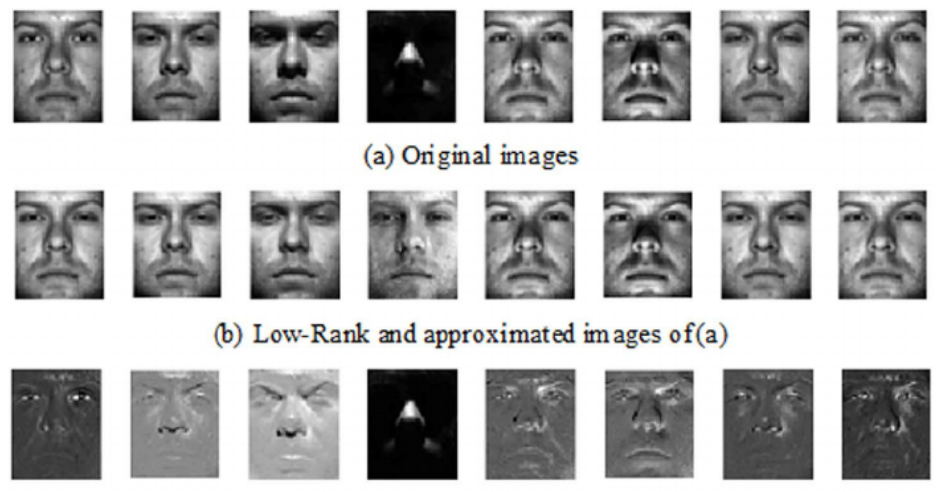
\includegraphics[width=\textwidth]{pca-example.png}
	\caption{Courtesy: Hou, Sun, Chong, Zheng 2014}
	\end{figure}
\end{frame}
\begin{frame}{PCA applied to Yale dataset}
	\begin{figure}
		\includegraphics[width=\textwidth]{pca-example-2.jpg}
	\caption{Courtesy: Shalev-Schwartz and Ben-David 2014}
	\end{figure}
\end{frame}

\begin{frame}{Linear algebra review: SVD}
	\begin{itemize}
		\item for any matrix $X \in \mathbb{R}^{m\times d}$, $X = U \Sigma V^\top$, where $U \in \mathbb{R}^{m\times m}$, $V \in \mathbb{R}^{d\times d}$ are orthogonal matrices, and $\Sigma \in \mathbb{R}^{m\times d}$ is a diagonal matrix.
		\pause
		\item $U$ and $V$ are the left and right singular vectors of $X$, and $\Sigma$ is the matrix of singular values of $X$.
		\pause
		\item $U$ and $V$ are the eigenvectors of $XX^\top$ and $X^\top X$ respectively.
		\pause
		\item $\Sigma$ is the square root of the eigenvalues of the SPSD matrices $X^\top X$ and $XX^\top$.
		

	\end{itemize}
\end{frame}
\begin{frame}{Eigenvalue decomposition, SPSD matrices, SVD}
\begin{itemize}
	\item for a square non-defective or diagonalizable matrix $A \in \mathbb{R}^{d\times d}$, $A = Q \Lambda Q^{-1}$, where $Q$ is the matrix of eigenvectors of $A$, and $\Lambda$ is the diagonal matrix of eigenvalues of $A$.
	\pause
	\item for an SPSD matrix, like $X X^\top$ or $X^\top X$, the eigenvalue decomposition is the same as SVD. Left and right singular vectors are the same and equal to the eigenvectors.
	\pause 
\item Reduced SVD: $X = U \Sigma V^\top$, where $U \in \mathbb{R}^{m\times r}$, $V \in \mathbb{R}^{d\times r}$ are orthogonal matrices, and $\Sigma \in \mathbb{R}^{r\times r}$ is a diagonal matrix (having non-zero values), when $X$ has rank $r$.
\end{itemize}
\end{frame}
\begin{frame}{SVD optimality}
	\begin{itemize}
		\item Geometric interpretation: if $S$ is the unit sphere in $\mathbb{R}^d$, $XS$ is the ellipsoid in $\mathbb{R}^m$. The vectors $\sigma_i u_i$ are the semi-axes of the ellipsoid; $v_i$ are the pre-images, i.e., $Xv_i = \sigma_i u_i$.
	\pause
	\item Theorem 5.8 (Trefethen and Bau): For any $k$-dimensional subspace $W$, the best rank-$k$ approximation to $X$ is given by $X_k = \sum_{i=1}^k \sigma_i u_i v_i^\top$. That is, 
	$$ {\rm arg min}_{\hat{X}: {\rm rank}(\hat{X})\leq k } \|X - \hat{X}\|_F =  {\rm arg min}_{\hat{X}: {\rm rank}(\hat{X})\leq k } \|X - \hat{X}\| =  X_k.$$
	\end{itemize}
\end{frame}
\begin{frame}{Rayleigh Quotient}
\begin{itemize}
	\item For a square matrix $A \in \mathbb{R}^{d\times d},$ the Rayleigh quotient is a scalar function,
	\begin{align*}
		r(x) = \frac{x^\top A x}{x^\top x}.
	\end{align*}
	\pause
	\item Eigenvalues of $A$ are the stationary points of $r(x)$.
	\pause
	\item $\nabla r(x) = \frac{2}{x^\top x} (Ax - r(x)x)$.
\end{itemize}
\end{frame}
\begin{frame}{PCA by SVD}
	\begin{itemize}
		\item When $m > d,$ do eigenvalue decomposition of $X^\top X$ or SVD of $X$.
		\pause
		\item When $m < d,$ do eigenvalue decomposition of $XX^\top.$ If $v_1, v_2,\cdots, v_n$ are the $n$ largest eigenvectors, principal vectors are $\frac{1}{\|X^\top v_i\|} X^\top v_i$.
		\pause
		\item Computational complexity: $O(\min(m^2d, md^2))$.

	\end{itemize}

\end{frame}
\end{document}
